% Shared AAAI body. \AnonSubmission toggles named/anonymous artefact links.
\newtheorem{theorem}{Theorem}
\newtheorem{proposition}{Proposition}
\newtheorem{definition}{Definition}
\newtheorem{corollary}{Corollary}

\title{Dynamic Trajectory Signatures: Physics-Guided Temporal Features for Data-Scarce Skeleton Fall Detection}

\author{Rudra Chopra}
\affiliations{Independent Researcher\\rudrachopra023@gmail.com}

\begin{document}
\maketitle

\begin{abstract}
When event dynamics are known and labelled data are scarce, principled temporal feature engineering can be theoretically motivated and empirically strong. We introduce the Dynamic Trajectory Signature (DTS), a 128-dimensional representation built from eight kinematically grounded skeleton primitives, each summarised by 16 temporal operators including temporal asymmetry: the fraction of a primitive's total path variation concentrated in the first $\tau$ of the sequence. DTS instantiates a \emph{physics-guided temporal signature} (PGTS) recipe that we hypothesise generalises to other data-scarce temporal events. We derive the Bayes-optimal scalar rule under an empirically supported Gaussian QDA model ($\varepsilon^{*}_{\mathrm{QDA}}=0.278$, training data only), prove a finite-sample separation theorem for the asymmetry statistic, and prove that any order-invariant feature is exactly at chance on a family of temporal-order constructions that DTS solves. Under a strict feature-group twin-free protocol with validation-only selection, DTS+HGB matches the strongest learned baselines, MultiROCKET and InceptionTime, from a 128-dimensional representation with zero sequence-learning parameters. It significantly outperforms the Transformer, MiniROCKET, a TCN, and both ST-GCN baselines, and posts the highest point-estimate AUROC among the fourteen target-trained models (0.9895 [0.9851, 0.9935] on 1,115 held-out FallVision clips). Against MiniROCKET the operating-point margin is large (recall 0.941 vs 0.861 at 5\% test FPR; 0.796 vs 0.629 at 1\%); MultiROCKET leads at the strictest budgets while DTS+HGB misses fewer falls at the F1 point (18 vs 32). Leave-session-out gives mean AUROC 0.9649, leave-fall-origin 0.8961, and zero-shot transfer holds up on URFD (0.9200) and the uncontrolled-home GMDCSA-24 (0.9633). Under true leave-one-subject-out on GMDCSA-24, DTS+HGB is comparable to MultiROCKET (0.941 vs 0.934, $n{=}4$ subjects). All artefacts and a numbers audit are released for one-command reproduction.
\end{abstract}

\section{Introduction}
A central question in machine learning is whether task-specific inductive bias, encoded as handcrafted features, can replace the representational power of deep models. For skeleton-based action recognition the dominant answer has been no: ST-GCN \citep{yan2018stgcn}, directed-graph variants \citep{shi2019directed}, and PoseC3D \citep{duan2022posec3d} achieve state-of-the-art results on large multi-class benchmarks, where end-to-end deep learning consistently outperforms handcrafted pipelines.

We identify two necessary conditions for this dominance: (i) the discriminative structure of the task is unknown a priori and must be learned; and (ii) enough labelled examples exist to regularise a competitive sequence model. When both fail simultaneously, we claim, principled feature engineering can be more data-efficient and achieve stronger AUROC than the evaluated sequence-learning baselines.

The contribution is not that falls can be detected with handcrafted features. The contribution is a testable claim about inductive bias in data-scarce temporal learning: when event dynamics are known, a fixed temporal-signature map can remove the burden of learning temporal structure from a generic sequence model. We name the underlying recipe \emph{physics-guided temporal signatures} (PGTS): name task primitives from the event mechanism, apply a fixed bank of temporal operators including an order-sensitive asymmetry statistic, select the single split parameter $\tau$ on training data only, and train a lightweight classifier. The Dynamic Trajectory Signature (DTS) studied here is PGTS instantiated for skeleton-based fall detection, and the paper tests the claim through strict leakage-proof evaluation, low-data learning curves, fixed-false-positive-rate operation, external transfer, subject-held-out validation, and a provably order-only benchmark family.

Continuous skeleton-based fall monitoring is attractive for elderly care because it is contactless and privacy-preserving, which makes fall detection a natural testbed for this claim. Falls have a kinematically distinctive three-phase structure (pre-fall stillness, a concentrated downward transition, horizontal rest) that is formally known rather than latent, and training data are scarce: FallVision \citep{fallvision2024} yields 5,793 usable clips after parsing, far below the scale on which ST-GCN was validated. DTS comprises eight kinematic primitives, each summarised by 16 temporal operators; the central operator is temporal asymmetry $\alpha(z;\tau)$ (Definition~\ref{def:alpha}), the fraction of a primitive's total path variation concentrated in the first $\tau$ of the sequence.

\textbf{Contributions.}
\begin{enumerate}
\item \textbf{Theory: Bayes bound, impossibility, and finite-sample separation.} Theorem~\ref{thm:qda} derives the Bayes-optimal rule for temporal asymmetry under the unequal-variance Gaussian model supported by Levene's test on training data ($p=5.3{\times}10^{-16}$), giving $\varepsilon^{*}_{\mathrm{QDA}}=0.278$. Theorem~\ref{thm:impossibility} proves any order-invariant feature is at chance on permutation-paired temporal-order constructions. Theorem~\ref{thm:finite} gives a finite-sample guarantee: thresholding $\alpha$ separates three-phase events from permuted negatives with failure probability decaying exponentially in sequence length.
\item \textbf{A strict twin-free evaluation protocol.} We document and correct a duplicated-extraction flaw in an earlier draft, deduplicate by feature fingerprint, and re-evaluate every model with validation-only selection, fixed seeds, saved score vectors, bootstrap intervals, and a released numbers audit.
\item \textbf{Competitive accuracy at a fraction of the representation cost.} A 128-dimensional DTS vector with gradient-boosted trees matches the strongest learned baselines (MultiROCKET and InceptionTime), significantly outperforms the recurrent, Transformer, TCN, and ST-GCN baselines, and dominates MiniROCKET at every false-alarm budget, while remaining markedly more sample-efficient.
\item \textbf{Robustness under distribution shift.} Subject-proxy and leave-fall-origin folds, zero-shot transfer to URFD and the uncontrolled-home GMDCSA-24, and true leave-one-subject-out on GMDCSA-24 all hold up; the one hard fold (Bed) is predicted by the QDA model and recovered by few-shot adaptation.
\item \textbf{An expanded construction-based test of temporal necessity.} On three controlled temporal-order constructions (three-phase falls, sit-to-stand ramps, direction-of-time reversal) whose negatives are frame permutations or reversals of positives, DTS attains AUROC $\geq0.99$ while order-invariant features remain exactly at chance; sweeps over noise, timing, duration, length, distractors, and operator subsets verify the theory's boundary conditions.
\end{enumerate}

\textbf{Scope.} Baselines span sequence models (LSTM, GRU, Transformer), compact and full COCO-adapted ST-GCNs, and MiniROCKET; PoseC3D \citep{duan2022posec3d} and pretrained systems are not evaluated, so superiority claims cover the evaluated baselines only. FallVision subject IDs are not public, so leave-session-out is used there only as a subject proxy; true leave-one-subject-out evaluation is reported separately on GMDCSA-24, which publishes subject identifiers. The sub-3\,ms runtime covers DTS extraction and inference only, excluding pose estimation.

\section{Related Work}
\textbf{Skeleton-based action recognition.} ST-GCN \citep{yan2018stgcn} established graph convolution over joint adjacency as the standard baseline; directed-graph variants \citep{shi2019directed}, MS-G3D \citep{liu2020msg3d}, CTR-GCN \citep{chen2021ctrgcn}, HD-GCN \citep{lee2023hdgcn}, and PoseC3D \citep{duan2022posec3d} improve multi-class benchmarks with abundant data, consistently outperforming handcrafted pipelines at scale. Pretrained 3D-CNN pose models such as PoseConv3D are increasingly used for few-shot fine-tuning; we treat pretraining as out of scope because it reintroduces the large-data condition our study isolates, and revisit it as future work. DTS instead encodes fall-specific structure explicitly for the binary, data-scarce regime.

\textbf{Pose-based fall detection.} \citet{lin2021robot} reach 97--98\% on URFD with recurrent models trained on URFD; \citet{zhu2025fall} report ST-GCN F1 0.962 with UR-Fall training. Our URFD result is zero-shot. Surveys identify device and environment shift as persistent failure modes \citep{igual2013challenges,mubashir2013survey,demiguel2017home}.

\textbf{Time-series classification baselines.} ROCKET \citep{dempster2020rocket}, MiniROCKET \citep{dempster2021minirocket}, and MultiROCKET \citep{tan2022multirocket} are among the strongest general-purpose time-series classifiers; InceptionTime \citep{fawaz2020inceptiontime} and temporal convolutional networks \citep{bai2018tcn} are the standard deep alternatives. We evaluate MiniROCKET, MultiROCKET, InceptionTime, and a TCN on the main split (the ROCKET variants via aeon \citep{middlehurst2024aeon} on the raw multivariate keypoint sequences), MultiROCKET additionally under subject-held-out transfer, and MiniROCKET under few-shot Bed adaptation.

\textbf{Inductive bias, data scarcity, and operating points.} Task-specific inductive bias helps in data-scarce regimes in medical signal processing \citep{rajpurkar2017cardiologist} and anomaly detection \citep{pang2021anomaly}, and structured biases are a recurring route to sample efficiency \citep{battaglia2018relational}. Distribution shift and the gap between ranking quality and calibrated operating points \citep{guo2017calibration,gulrajani2021domain} motivate our fixed-FPR, transfer, and threshold-shift analyses.

\section{Theory: Temporal Asymmetry, Impossibility, and Finite-Sample Separation}
\begin{definition}[Temporal Asymmetry Operator]\label{def:alpha}
For a scalar primitive trajectory $z=z_{1:T}$ and split $\tau\in(0,1)$, let $\Delta z_t = z_t - z_{t-1}$. Define
\begin{equation}
\alpha(z;\tau)=\frac{\sum_{t=2}^{\lfloor \tau T\rfloor}|\Delta z_t|}{\sum_{t=2}^{T}|\Delta z_t| + \epsilon},
\label{eq:alpha}
\end{equation}
where $\epsilon=10^{-8}$ is a fixed numerical stabiliser used only to avoid division by zero for degenerate trajectories with no motion.
\end{definition}
Falls concentrate motion in the transition phase (small $\alpha$); non-falls distribute variation more evenly (larger $\alpha$).

\begin{theorem}[QDA Bayes Bound for Temporal Asymmetry]\label{thm:qda}
Let $\alpha \mid c \sim \mathcal{N}(\mu_c,\sigma_c^2)$, $c\in\{f,n\}$, with equal priors. Under the heteroscedastic model ($\sigma_f\neq\sigma_n$), the Bayes-optimal classifier is a quadratic discriminant rule with two real crossover points $x_1<x_2$ satisfying
\begin{equation}
\Big(\tfrac{1}{\sigma_f^2}-\tfrac{1}{\sigma_n^2}\Big)x^2
-2\Big(\tfrac{\mu_f}{\sigma_f^2}-\tfrac{\mu_n}{\sigma_n^2}\Big)x
+\Big(\tfrac{\mu_f^2}{\sigma_f^2}-\tfrac{\mu_n^2}{\sigma_n^2}\Big)-2\ln\tfrac{\sigma_n}{\sigma_f}=0.
\label{eq:qda}
\end{equation}
Fall is assigned to the interior $(x_1,x_2)$ when $\sigma_f<\sigma_n$. The Bayes error is
$\varepsilon^{*}_{\mathrm{QDA}}=\tfrac12\big(P(\alpha\notin(x_1,x_2)\mid f)+P(\alpha\in(x_1,x_2)\mid n)\big)$.
\end{theorem}

\begin{proposition}[Empirical QDA Bound on FallVision]\label{prop:empirical}
For the hip-speed primitive at $\tau^{*}=0.30$, estimated on the corrected twin-free \emph{training split only} (3,565 clips): $\hat\mu_f=0.162$, $\hat\sigma_f=0.169$, $\hat\mu_n=0.381$, $\hat\sigma_n=0.209$. Levene's test strongly rejects equal variance ($p=5.3{\times}10^{-16}$), supporting the QDA form over an equal-variance LDA approximation. Equation~\eqref{eq:qda} yields $x_1\approx-0.80$ and $x_2\approx 0.293$, with $P(\mathrm{miss}\mid f)=0.219$ and $P(\mathrm{false\ alarm}\mid n)=0.337$, so $\varepsilon^{*}_{\mathrm{QDA}}=0.278$. The full eight-family DTS reduces the observed held-out error to 0.051, a factor-5.5 reduction relative to this single-primitive bound.
\end{proposition}
Because $\alpha\in[0,1)$ by construction, the lower crossover $x_1\approx-0.80$ lies outside the support, and the effective decision rule on FallVision is the single threshold $x_2\approx0.293$.

\begin{theorem}[Order-Invariance Impossibility]\label{thm:impossibility}
Let a clip be $x=(x_1,\dots,x_T)\in(\mathbb{R}^d)^T$, and call a feature map $\phi$ order-invariant if $\phi(x_{\sigma(1)},\dots,x_{\sigma(T)})=\phi(x)$ for every permutation $\sigma\in S_T$. Consider any temporal-order construction in which each negative is generated as $X^-=\sigma(X^+)$ with $X^+\sim P_+$ and $\sigma$ a (possibly random) permutation independent of $X^+$. Then for any classifier $g=h\circ\phi$ built on an order-invariant $\phi$, the class-conditional score laws coincide, $g(X^-)\stackrel{d}{=}g(X^+)$; hence the ROC curve is the diagonal, $\mathrm{AUROC}=\tfrac12$, and the Bayes error is $\tfrac12$.
\end{theorem}
Theorem~\ref{thm:impossibility} is elementary, but it fixes the exact-chance boundary that no order-blind representation can cross (the appendix proof is pointwise in $\sigma$, covering both random permutations and exact time reversal, and matches the bag-of-frames classifier in Figure~\ref{fig:benchmark}). An order-sensitive statistic escapes this bound, now in finite-sample form:

\begin{theorem}[Finite-Sample Asymmetry Separation]\label{thm:finite}
Model a fall primitive by $n$ independent increment magnitudes $w_t\in[0,B]$ with mean $\mu_s$ on a still phase $t/n\in[0,p_1)$ and floor phase $[p_2,1]$, and mean $\mu_d\geq\mu_s$ on the drop phase $[p_1,p_2)$; let the matched negative be a uniformly random permutation of the same increments. Fix $\tau\leq p_1$ and let $\bar\mu=(p_1{+}1{-}p_2)\mu_s+(p_2{-}p_1)\mu_d$, $a_f=\tau\mu_s/\bar\mu$, and the asymmetry gap $\Delta=\tau-a_f=\tau(p_2{-}p_1)(\mu_d{-}\mu_s)/\bar\mu>0$. Then for all $n\geq 6/\Delta$, the threshold rule ``fall iff $\alpha\leq\theta$'' with $\theta=a_f+\Delta/2$ satisfies
\begin{equation}
P(\alpha_{\mathrm{fall}}\geq\theta)+P(\alpha_{\mathrm{neg}}\leq\theta)\;\leq\;5\exp\!\Big(-\frac{n\,\bar\mu^{2}\Delta^{2}}{72\,B^{2}}\Big),
\label{eq:finite}
\end{equation}
and consequently $\mathrm{AUROC}(\alpha)\geq 1-5\exp\!\big(-n\bar\mu^2\Delta^2/(72B^2)\big)$ and the balanced misclassification error of the threshold rule is at most $\tfrac52\exp\!\big(-n\bar\mu^2\Delta^2/(72B^2)\big)$.
\end{theorem}

The proof (appendix) uses Hoeffding's inequality on the fall windows and Hoeffding--Serfling concentration for sampling without replacement on the permuted negative \citep{hoeffding1963,serfling1974}; a corollary extends the guarantee to majority votes over $k$ independent primitives. Constants are not optimised; in simulation the failure probability decays exponentially in $n$ with far better constants (verification script released). The model is an idealisation that formalises the mechanism DTS exploits and is tested directly by the controlled benchmark, and it makes the sample-length condition explicit (error $\leq\delta$ once $n\geq \frac{72B^2}{\bar\mu^2\Delta^2}\ln\frac{5}{\delta}$), quantifying when a single fixed statistic suffices.

\section{Dynamic Trajectory Signature}
\subsection{Preprocessing}
Skeleton sequences $S\in\mathbb{R}^{T\times17\times2}$ are hip-centred (midpoint of COCO joints 11--12) and torso-normalised (median shoulder-to-hip distance). Missing keypoints are linearly interpolated, and keypoints with confidence below 0.10 are zeroed.

\subsection{Primitives and Feature Extraction}
Eight primitives are extracted per clip: bounding-box width, hip-centre height, torso angle, hip speed, centre-of-mass speed, hip acceleration, shoulder height, and head height. Each primitive $z\in\mathbb{R}^{T}$ receives the 16-dimensional operator
\begin{align*}
\Omega(z;\tau)=[\,&\mu,\sigma,\min,\max,Q_{25},Q_{50},Q_{75},R,z_1,z_T,\\
&\delta,\beta,\textstyle\sum|\Delta z|,|\Delta z|_{\max},|\Delta^2 z|_{\max},\alpha(z;\tau)\,],
\end{align*}
yielding a fixed $\phi(X)\in\mathbb{R}^{128}$ representation.

\subsection{Optimal Split $\tau^{*}$}
$\tau^{*}$ maximises the summed two-sample Welch $t$-statistic over all eight primitives on the training split, using a 13-point grid on $[0.20,0.80]$. On FallVision, $\tau^{*}=0.30$; on URFD, the FallVision value is used without retuning. The result is consistent with an initial stillness phase in fall clips followed by late, concentrated motion.

\subsection{DTS-Net: Interpretable Neural Variant}
DTS-Net applies asymmetry-guided softmax attention over the eight feature blocks followed by an MLP ($128{\rightarrow}64{\rightarrow}32{\rightarrow}1$) with an auxiliary asymmetry-regression loss ($\lambda=0.15$; 10,506 parameters); it provides an exploratory attention view of family salience, while tree ensembles provide peak accuracy.

\subsection{The General Recipe: Physics-Guided Temporal Signatures}
DTS instantiates a five-step recipe: (1) name task primitives from the event mechanism; (2) derive a fixed temporal operator bank, including an asymmetry statistic; (3) estimate $\tau^{*}$ from training data only; (4) train a lightweight classifier; (5) validate under low-data and domain-shift protocols. We \emph{hypothesise} that this recipe extends to other events with a characterisable temporal profile (sit-to-stand, lying transitions, near-falls, gait-phase); falls are the only real-data instance here, so generality beyond fall detection is a conjecture this paper motivates, not establishes (the controlled benchmark offers preliminary support on two synthetic profiles).

\section{Experimental Setup}
\subsection{Data, Deduplication, and Splits}
Parsing the FallVision keypoint archives yields 5,793 clips (2,966 falls, 2,827 non-falls) across three acquisition groups (Bed, Chair, Stand) and four session identifiers. An earlier draft of this work was evaluated on a faulty archive extraction in which each clip appeared three to four times under different archive labels, and 728 duplicated clips straddled the train/test boundary; every headline result in that draft was inflated by this leakage.\footnote{For example, the earlier draft reported held-out AUROC 0.9998 and recall 1.000 for DTS+HGB; the strict twin-free protocol yields 0.9895 and 0.969. The corrected numbers supersede all previously circulated results.} All main results use a strict feature-group twin-free protocol: clips are grouped by feature fingerprint, identical-feature groups with conflicting labels dropped (none here), one representative kept per group (5,572 representatives; 221 duplicate members removed), then stratified 64/16/20 into 3,565 train, 892 validation, and 1,115 test clips (574 falls, 541 non-falls), guaranteeing no feature-identical twin straddles the splits. Leave-session-out and leave-fall-origin use the same 5,572 representatives. URFD \citep{kwolek2014urfd} provides 30 falls and 40 activities of daily living, used only for zero-shot transfer. Throughout, \emph{target-trained} denotes models trained exclusively on the FallVision training split, with no external pretraining.

\subsection{Baselines}
\textbf{Neural sequence models.} A 2-layer LSTM (hidden size 128; 216,193 parameters), a 2-layer GRU (hidden size 128), and a temporal Transformer (4 heads, 2 layers, $d_{\mathrm{model}}=64$), trained on normalised keypoint sequences of shape $(T,34)$.

\textbf{Graph baselines.} Compact ST-GCN (244,161 parameters) and a deeper FullST-GCN-COCO (1,107,905 parameters), both using the 17-node COCO adjacency and temporal graph-convolution blocks adapted from ST-GCN \citep{yan2018stgcn}, trained from scratch on FallVision.

\textbf{Convolutional time-series baselines.} MiniROCKET \citep{dempster2021minirocket} via aeon \citep{middlehurst2024aeon} on the same hip-centred, torso-normalised 34-channel sequences (fixed maximum length 150), and MultiROCKET \citep{tan2022multirocket} (49,728 features; ridge with validation-selected regularisation).

\textbf{Deep convolutional baselines} (JAX \citep{jax2018}). A four-block dilated causal TCN \citep{bai2018tcn} (dilations 1--8, 64 channels, 43,713 parameters) and a \emph{resource-matched} InceptionTime \citep{fawaz2020inceptiontime}: a three-network ensemble of depth-6 Inception networks (bottleneck 32, kernels 40/20/10, 496,129 parameters each; probabilities averaged), trained under the same 20-epoch budget as the other neural baselines rather than the canonical five-network, train-to-convergence setup. Both use Adam, gradient clipping, and validation-AUROC checkpointing.

\textbf{Harness fidelity.} The added baselines consume sequences rebuilt from the raw archives via the released manifest; the rebuild reproduces DTS+HGB's AUROC (0.9895, exact) and MiniROCKET's (0.9797, within its published interval; the residual difference is attributable to ridge-regularisation selection, validation-selected here versus leave-one-out in the original run, and library version, the MiniRocket transform being deterministic at fixed seed).

\textbf{DTS classifiers.} Logistic regression, ExtraTrees, random forest, and HistGradientBoosting on the 128-dimensional DTS vector; DTS-Net as above.

\subsection{Hyperparameter Selection and Training Protocol}
All model selection uses the validation split only; test labels are never used for any selection step. DTS classifiers use a grid search selected on validation AUROC with an F1 tie-break (grids in Appendix Table~\ref{tab:grids}); decision thresholds for every model maximise validation F1 on $[0.01,0.99]$; MiniROCKET's kernel count is selected on validation AUROC over $\{1{,}000;5{,}000;10{,}000\}$ (10,000 chosen). Neural and graph baselines train with AdamW ($10^{-3}$, weight decay $10^{-4}$), gradient clipping 1.0, validation-AUROC checkpointing, 20 epochs (FullST-GCN-COCO: 24 epochs, batch 48; DTS-Net: 40 epochs at $3{\times}10^{-3}$). All runs use fixed seeds; released result files record every grid, configuration, threshold, score vector, and split manifest.

\subsection{Confidence Intervals}
All intervals are 95\%. AUROC and threshold metrics use nonparametric bootstrap intervals (1,000 resamples, fixed seed) from saved test score vectors; summary-only count metrics (including URFD recall) use Wilson intervals; the URFD AUROC interval uses the Hanley--McNeil method (no score vector was retained from the archived legacy run); FP/FN are deterministic counts. Pairwise comparisons use a paired bootstrap on the AUROC difference over identical resamples; the five comparisons against DTS+HGB are pre-specified and remain significant after Bonferroni correction (99\% paired intervals also exclude zero).

\section{Results}
\subsection{Main Held-Out Performance}
Table~\ref{tab:main} presents the central result on the strict twin-free split. DTS+HGB attains AUROC 0.9895 [0.9851, 0.9935] and F1 0.951 [0.938, 0.963] with 18 missed falls, the highest point-estimate AUROC among the fourteen evaluated target-trained models under this protocol. The five pre-specified paired-bootstrap comparisons are all significant in favour of DTS+HGB: +0.0183 [0.0105, 0.0266] versus GRU, +0.0085 [0.0024, 0.0151] versus Transformer, +0.0135 [0.0058, 0.0220] versus MiniROCKET, +0.0710 [0.0568, 0.0879] versus Compact ST-GCN, and +0.0242 [0.0166, 0.0338] versus FullST-GCN-COCO. The added baselines (MultiROCKET, InceptionTime, TCN) are additional, non-prespecified paired comparisons, reported with uncorrected 95\% intervals: DTS+HGB significantly outperforms the TCN (+0.0265 [0.0163, 0.0377]; still significant under Bonferroni across the expanded eight-comparison family, [0.0131, 0.0422]) and \emph{matches} the two strongest, MultiROCKET (0.9868 [0.9808, 0.9920]; +0.0027 [$-$0.0035, 0.0086]) and InceptionTime (0.9834 [0.9774, 0.9889]; +0.0061 [$-$0.0002, 0.0123]), neither margin significant before or after correction. DTS uses a 128-dimensional representation, against MultiROCKET's 49,728 transform features and InceptionTime's $\sim$1.5M-parameter ensemble, and misses the fewest falls at the F1 operating point (18 vs 32 and 44).

\begin{table*}[t]
\centering
\small
\setlength{\tabcolsep}{1.8pt}
\begin{tabular}{lccccccc}
\toprule
Model & AUROC & F1 & Precision & Recall & Accuracy & FP & FN \\
\midrule
LSTM & 0.9558 [0.9446, 0.9662] & 0.905 [0.886, 0.920] & 0.893 [0.866, 0.917] & 0.916 [0.894, 0.937] & 0.900 [0.883, 0.917] & 63 & 48 \\
GRU & 0.9712 [0.9623, 0.9795] & 0.920 [0.903, 0.937] & 0.913 [0.890, 0.936] & 0.927 [0.905, 0.946] & 0.917 [0.900, 0.934] & 51 & 42 \\
Transformer & 0.9810 [0.9749, 0.9872] & 0.940 [0.926, 0.954] & 0.947 [0.929, 0.964] & 0.934 [0.913, 0.953] & 0.939 [0.925, 0.952] & 30 & 38 \\
Compact ST-GCN & 0.9185 [0.9016, 0.9340] & 0.849 [0.826, 0.870] & 0.851 [0.822, 0.879] & 0.847 [0.816, 0.877] & 0.845 [0.823, 0.865] & 85 & 88 \\
FullST-GCN-COCO & 0.9652 [0.9553, 0.9740] & 0.907 [0.889, 0.924] & 0.895 [0.868, 0.919] & 0.920 [0.896, 0.941] & 0.903 [0.885, 0.920] & 62 & 46 \\
MiniROCKET & 0.9760 [0.9672, 0.9839] & 0.936 [0.921, 0.950] & 0.931 [0.910, 0.952] & 0.941 [0.920, 0.960] & 0.934 [0.918, 0.948] & 40 & 34 \\
MultiROCKET$^{\dagger}$ & 0.9868 [0.9808, 0.9920] & 0.949 [0.935, 0.962] & 0.954 [0.937, 0.971] & 0.944 [0.924, 0.963] & 0.948 [0.935, 0.961] & 26 & 32 \\
InceptionTime$^{\dagger}$ & 0.9834 [0.9774, 0.9889] & 0.941 [0.927, 0.956] & 0.960 [0.944, 0.975] & 0.923 [0.900, 0.946] & 0.941 [0.927, 0.954] & 22 & 44 \\
TCN$^{\dagger}$ & 0.9629 [0.9523, 0.9734] & 0.910 [0.893, 0.928] & 0.893 [0.868, 0.916] & 0.929 [0.909, 0.950] & 0.906 [0.889, 0.923] & 64 & 41 \\
\midrule
DTS+LR & 0.9433 [0.9297, 0.9559] & 0.890 [0.871, 0.909] & 0.883 [0.858, 0.906] & 0.897 [0.874, 0.922] & 0.886 [0.867, 0.905] & 68 & 59 \\
DTS+ET & 0.9801 [0.9734, 0.9861] & 0.936 [0.921, 0.950] & 0.907 [0.883, 0.931] & 0.967 [0.952, 0.980] & 0.932 [0.917, 0.946] & 57 & 19 \\
DTS+RF & 0.9785 [0.9711, 0.9849] & 0.927 [0.912, 0.941] & 0.893 [0.870, 0.917] & 0.963 [0.946, 0.978] & 0.922 [0.906, 0.937] & 66 & 21 \\
DTS+HGB & \textbf{0.9895} [0.9851, 0.9935] & \textbf{0.951} [0.938, 0.963] & 0.934 [0.913, 0.954] & 0.969 [0.953, 0.983] & \textbf{0.949} [0.935, 0.961] & 39 & 18 \\
DTS-Net & 0.9775 [0.9699, 0.9849] & 0.928 [0.911, 0.943] & 0.927 [0.907, 0.949] & 0.929 [0.907, 0.949] & 0.926 [0.909, 0.941] & 42 & 41 \\
\bottomrule
\end{tabular}
\caption{FallVision held-out results on the strict twin-free test split: 1,115 clips (574 falls, 541 non-falls). Brackets are 95\% confidence intervals; AUROC is reported to four decimal places and all other metrics to three; FP and FN are deterministic counts. Thresholds are tuned on validation F1 for every model. $^{\dagger}$Reviewer-requested baselines added on identically rebuilt sequences under the same validation-only protocol (harness fidelity: rebuilt DTS features reproduce DTS+HGB AUROC 0.9895 exactly; MiniROCKET re-run in this harness gives 0.9797, within its published interval). InceptionTime is a resource-matched three-network ensemble (see Baselines).}
\label{tab:main}
\end{table*}

At the validation-F1 operating point, DTS+HGB also has a favourable threshold trade-off: 18 false negatives and 39 false positives versus MiniROCKET's 34 and 40.

\textbf{Why DTS performs well here.} Three consistent factors: the QDA-optimal $\alpha$ statistic (Theorem~\ref{thm:qda}); low capacity relative to the training set (appendix heuristic); and long-range temporal coverage by slope, asymmetry, and acceleration summaries that sequence models must infer from limited data.

\subsection{Operating Points: Recall at Fixed False-Positive Rate}
For deployment, the relevant question is recall at an acceptable alarm rate: continuous monitoring systems are abandoned when false alarms are frequent, so a model with lower false-positive burden at fixed recall can be more usable than one with similar AUROC but worse low-FPR behaviour. Table~\ref{tab:fpr} reports recall at test false-positive rates of 1\%, 2\%, 5\%, and 10\%. DTS+HGB dominates MiniROCKET at every constraint (0.796 [0.761, 0.827] vs 0.629 [0.589, 0.667] at a strict 1\% FPR), where ranking-quality differences translate directly into missed-fall reductions. Against MultiROCKET the result is split: MultiROCKET recalls more falls at the strictest budgets (0.864 vs 0.796 at 1\%; 0.882 vs 0.862 at 2\%), the two tie at 5\% (0.944 vs 0.941), and DTS+HGB leads at 10\% (0.981 vs 0.977) and at the validation-F1 operating point (18 vs 32 missed falls). With AUROC indistinguishable, the choice between them is a deployment decision; DTS+HGB adds interpretability, a 128-dimensional representation versus MultiROCKET's 49,728 transform features (a representation-size contrast, not a clean efficiency ratio: MultiROCKET's features can be sparse and its transform is optimised), and sub-3\,ms CPU inference.

\begin{table}[t]
\centering
\small
\setlength{\tabcolsep}{2.6pt}
\begin{tabular}{lccc}
\toprule
Max FPR & DTS+HGB & MiniROCKET & MultiROCKET$^{\dagger}$ \\
\midrule
1\% & 0.796\,{\scriptsize[0.761,\,0.827]} & 0.629\,{\scriptsize[0.589,\,0.667]} & \textbf{0.864}\,{\scriptsize[0.834,\,0.890]} \\
2\% & 0.862\,{\scriptsize[0.832,\,0.888]} & 0.777\,{\scriptsize[0.741,\,0.809]} & \textbf{0.882}\,{\scriptsize[0.853,\,0.905]} \\
5\% & 0.941\,{\scriptsize[0.918,\,0.957]} & 0.861\,{\scriptsize[0.830,\,0.887]} & \textbf{0.944}\,{\scriptsize[0.922,\,0.960]} \\
10\% & \textbf{0.981}\,{\scriptsize[0.966,\,0.989]} & 0.970\,{\scriptsize[0.953,\,0.981]} & 0.977\,{\scriptsize[0.962,\,0.987]} \\
\bottomrule
\end{tabular}
\caption{Recall at fixed test false-positive rate on the strict twin-free FallVision split (1,115 clips; 95\% Wilson intervals). DTS+HGB dominates MiniROCKET everywhere; the added MultiROCKET leads at the strictest budgets while DTS+HGB leads at 10\% and at the F1 point, with statistically indistinguishable AUROC.}
\label{tab:fpr}
\end{table}

\subsection{Sample Efficiency on Real Data}
The data-scarcity claim is tested directly by retraining on stratified subsamples of the strict twin-free training set ($n\in\{250,500,1{,}000,2{,}000,3{,}565\}$; validation, test set, and protocol unchanged) for DTS+HGB and the three strongest baselines (Transformer, MiniROCKET, and MultiROCKET, the last refit per subsample). As Figure~\ref{fig:sampleeff} shows, DTS+HGB dominates the Transformer and MiniROCKET at every size, with the largest margins in the scarcest regimes, and tracks MultiROCKET throughout. A paired bootstrap finds no significant DTS$-$MultiROCKET difference at any size (all five 95\% intervals contain zero; Appendix Table~\ref{tab:lcpaired}); both are far more sample-efficient than the learned sequence models. This sweep, not the appendix capacity heuristic, is the main support for the data-efficiency claim.

\begin{figure}[t]
\centering
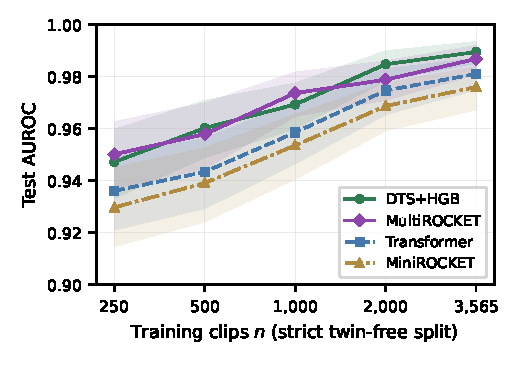
\includegraphics[width=0.96\columnwidth]{fig1_sample_efficiency.pdf}
\caption{Sample efficiency on the strict twin-free split: test AUROC versus training-set size for DTS+HGB, the strongest originally evaluated baselines (Transformer, MiniROCKET), and MultiROCKET (transform refit per subsample; shaded bands are 95\% bootstrap intervals; validation and test sets fixed). DTS+HGB dominates the Transformer and MiniROCKET at every size and tracks MultiROCKET within overlapping intervals.}
\label{fig:sampleeff}
\end{figure}

\subsection{Leave-Fall-Origin Robustness}
Across acquisition groups (Appendix Table~\ref{tab:lfo}, fixed threshold 0.5), Chair (AUROC 0.9844) and Stand (0.9916) transfer readily, while Bed (0.7123) is the one hard fold, as the scalar QDA analysis predicts: semi-reclined falls shift $\hat\mu_f,\hat\sigma_f$ outside the Chair+Stand support. We define the transfer gap $\Gamma_{F1}$ as the stratified-iid-reference F1 minus the leave-fall-origin mean F1: $\Gamma_{F1}=0.951-0.880=0.071$ (Appendix Figure~\ref{fig:lfopanels}). We diagnose and recover the Bed fold below.

\subsection{Zero-Shot Cross-Dataset Transfer}
DTS+HGB trained on FallVision and applied to URFD without retraining obtains AUROC 0.9200 [0.8483, 0.9917] and recall 1.000 [0.886, 1.000], detecting all 30 URFD falls at the fixed threshold (Table~\ref{tab:transfer}). With only 30 falls and 40 non-falls the intervals are wide; the perfect observed recall is not a precise population estimate. This experiment uses the archived FallVision-trained model and is unaffected by FallVision-internal duplication (URFD is external). The 29 false positives reflect a large score-calibration shift rather than poor ranking, since AUROC remains high; precision is 0.508 [0.384, 0.632], and the fixed-threshold false-positive rate is 0.725 (29/40). Without a URFD validation split we do not estimate a calibrated operating threshold.

\textbf{GMDCSA-24.} We apply the same archived model to GMDCSA-24 \citep{alam2024gmdcsa}, a 4-subject dataset recorded in natural home settings under varied lighting and a low-resolution webcam. Zero-shot DTS+HGB reaches AUROC 0.9633 on all 160 clips, and unlike URFD the default threshold is already usable (recall 0.924, precision 0.880; full table in Appendix Table~\ref{tab:transfer}). GMDCSA-24 also publishes subject identifiers, enabling the true subject-held-out test below.

\textbf{Score distributions.} Appendix Figure~\ref{fig:scoredists} visualises calibration from the saved score vectors: FallVision and GMDCSA-24 are cleanly separated at the default threshold (non-fall mass above 0.5: 7.2\% and 12.3\%); the Bed fold's high-score non-fall mass is partially cleared by adaptation. URFD vectors were not retained; its shift is quantified in the text (FPR 0.725 despite AUROC 0.9200).

\subsection{True Subject-Held-Out Evaluation}
FallVision publishes no subject IDs, so leave-session-out (Appendix Table~\ref{tab:lso}) is only a proxy; GMDCSA-24 publishes subject IDs, enabling genuine leave-one-subject-out (train three subjects, test the fourth). Appendix Table~\ref{tab:loso} compares DTS+HGB to a modern target-trained baseline, MultiROCKET \citep{tan2022multirocket}, MiniROCKET, and asymmetry-only logistic regression. DTS+HGB has the best mean AUROC (0.941) ahead of MultiROCKET (0.934), MiniROCKET (0.918), and asymmetry-only (0.917); the DTS$-$MultiROCKET margin (paired pooled out-of-fold AUROC $+0.012$ [$-0.034$, $0.056$]) is not significant at four subjects, so we state it as a match: a handcrafted 128-d representation matches a strong modern convolutional time-series baseline under person-level shift.

\subsection{Bed-Origin Failure: Diagnosis and Recovery}
The Bed fold is the one hard case (AUROC 0.7123 zero-shot, Appendix Table~\ref{tab:lfo}). We characterise and reduce it rather than hide it: it is a representation shift, not miscalibration (re-tuning the Bed threshold barely moves F1, so the gap is in ranking). Error analysis: missed Bed falls have higher hip-speed asymmetry ($\alpha\approx0.33$) than detected ones ($\alpha\approx0.21$), exactly the direction the QDA model predicts: semi-reclined falls have a shorter, less front-loaded descent. Few-shot recovery: adding $K$ labelled Bed clips to Chair+Stand training lifts Bed AUROC monotonically, from 0.714 at $K{=}0$ to 0.858 at $K{=}200$ (Appendix Figure~\ref{fig:bedorig}). Under an identical protocol for all three models (Figure~\ref{fig:bed}), DTS+HGB stays ahead of MiniROCKET at every budget and tracks the stronger MultiROCKET, mirroring the main-split and subject-held-out results. The failure is interpretable and largely closed with minimal target supervision.

\begin{figure}[t]
\centering

\includegraphics[width=0.88\columnwidth]{fig_bed_compare.pdf}
\caption{Few-shot Bed recovery under the identical protocol for all three models (mean$\pm$95\% interval over five seeds; fixed 1,547-clip Bed test, 200-clip adaptation pool). DTS+HGB adapts faster than MiniROCKET+ridge at every budget and is matched by the stronger MultiROCKET+ridge, which is marginally ahead throughout, mirroring the main-split and subject-held-out results.}
\label{fig:bed}
\end{figure}

\subsection{Feature Ablations}
Appendix Table~\ref{tab:ablation} reports single-family removal under the main protocol (each row retrained, threshold re-tuned on validation). No removal causes large degradation (largest AUROC drop $-0.0039$): DTS is intentionally over-complete, each family carrying partially redundant signal for robustness to missing or noisy keypoints. Zeroing all eight asymmetry elements costs only $-0.0023$ AUROC; this does not show $\alpha$ is unnecessary, because other operators (slopes, velocities, accelerations) encode correlated order information and absorb the signal; the controlled benchmark below isolates the pure ordering question.

\subsection{Expanded Controlled Temporal-Order Benchmark}
A synthetic benchmark family realises Theorem~\ref{thm:impossibility}'s assumptions exactly: three constructions (three-phase falls and sit-to-stand ramps with frame-permuted negatives; early-burst trajectories with exact time reversals) make class-conditional frame multisets identical, so only ordering carries label information. DTS+HGB and $\alpha$-only solve all three; order-invariant bag-of-frames and order-invariant operator subsets of DTS sit exactly at 0.500; $\alpha$-only degrades at SNR near 1 or under misspecified fixed $\tau$ while the full bank stays at ceiling (full tables, sweeps, and construction details in Appendix Tables~\ref{tab:bench}--\ref{tab:benchsweeps}).

\section{Discussion}
Principled feature engineering wins when task structure is formally characterisable, data are scarce relative to model capacity, and the bias matches the mechanism; all three hold here. It should fail when event structure is unknown, classes differ subtly, appearance cues dominate, or abundant data and pretrained models restore learned representations; we make no claim for large multi-class benchmarks or pretrained systems. URFD's false positives are a calibration, not ranking, shift; extraction and inference run in under 3\,ms per clip on CPU ($<$50\,MB).

\section{Limitations}
\textbf{Erratum.} An earlier draft's near-ceiling results were traced to duplicated clips leaking across splits; all numbers use the strict twin-free protocol (artefacts released). \textbf{Subject identity.} FallVision subject IDs are unpublished (leave-session-out is only a proxy); true subject-held-out evidence comes from GMDCSA-24, which has four subjects, so the LOSO comparison is underpowered and stated as a match. \textbf{Baselines.} ST-GCNs are trained from scratch; PoseC3D and pretrained or fine-tuned systems are not evaluated, since pretraining reintroduces the large-external-data regime we isolate, so comparisons are limited to the evaluated baselines. InceptionTime is reported under a resource-matched budget; the canonical five-network train-to-convergence configuration was not run for compute reasons and is left to future work, though a stronger InceptionTime would reinforce rather than threaten the matches-learned-models claim. \textbf{Domain shift.} Bed falls remain hardest (0.7123 zero-shot) and URFD needs threshold calibration; both are quantified, not solved; Bed recovery needs labelled target clips. \textbf{Population.} Subjects are healthy adults aged 22--27; elderly or frail-adult falls may violate the three-phase pattern more often. \textbf{Scope.} PGTS assumes known event mechanics and a low-dimensional discriminative signal, and is not expected to scale to large multi-class recognition; the sub-3\,ms runtime excludes pose estimation; and the DTS-Net attention weights are only suggestive and should not be read as an explanation.

\section{Conclusion}
Under the strict twin-free protocol, DTS+HGB matches MultiROCKET with a far smaller, interpretable representation and zero sequence-learning parameters, dominates MiniROCKET at every fixed FPR, and posts the highest point-estimate AUROC among the fourteen target-trained models (0.9895). When event mechanics are known and data are scarce, physics-guided temporal signatures are a strong and interpretable alternative, and the accompanying theory marks out where the approach should and should not work.

\ifnum\AnonSubmission=0
\section*{Acknowledgments}
James Begin (University of Waterloo) carefully reviewed the manuscript across multiple revisions and provided feedback that sharpened the framing and analysis.
\fi

% Shared bibliography (natbib-compatible, AAAI author-year format).
% All entries verified real; new entries added for the venue upgrades:
% InceptionTime, TCN, CTR-GCN, HD-GCN, calibration (Guo et al.), domain
% generalization (Gulrajani & Lopez-Paz), inductive bias (Battaglia et al.),
% Hoeffding 1963, Serfling 1974.
\begin{thebibliography}{30}
\providecommand{\natexlab}[1]{#1}

\bibitem[{Alam et~al.(2024)Alam, Sufian, Dutta, Leo, and Hameed}]{alam2024gmdcsa}
Alam, E.; Sufian, A.; Dutta, P.; Leo, M.; and Hameed, I.~A. 2024.
\newblock GMDCSA-24: A dataset for human fall detection in videos.
\newblock \emph{Data in Brief}, 57: 110892.

\bibitem[{Bai, Kolter, and Koltun(2018)}]{bai2018tcn}
Bai, S.; Kolter, J.~Z.; and Koltun, V. 2018.
\newblock An Empirical Evaluation of Generic Convolutional and Recurrent Networks for Sequence Modeling.
\newblock arXiv:1803.01271.

\bibitem[{Battaglia et~al.(2018)Battaglia, Hamrick, Bapst, et~al.}]{battaglia2018relational}
Battaglia, P.~W.; Hamrick, J.~B.; Bapst, V.; et~al. 2018.
\newblock Relational inductive biases, deep learning, and graph networks.
\newblock arXiv:1806.01261.

\bibitem[{Bradbury et~al.(2018)Bradbury, Frostig, Hawkins, Johnson, Leary, Maclaurin, Necula, Paszke, VanderPlas, Wanderman-Milne, and Zhang}]{jax2018}
Bradbury, J.; Frostig, R.; Hawkins, P.; Johnson, M.~J.; Leary, C.; Maclaurin, D.; Necula, G.; Paszke, A.; VanderPlas, J.; Wanderman-Milne, S.; and Zhang, Q. 2018.
\newblock JAX: composable transformations of Python+NumPy programs.
\newblock \url{http://github.com/google/jax}.

\bibitem[{Chen et~al.(2021)Chen, Zhang, Yuan, Li, Deng, and Hu}]{chen2021ctrgcn}
Chen, Y.; Zhang, Z.; Yuan, C.; Li, B.; Deng, Y.; and Hu, W. 2021.
\newblock Channel-wise Topology Refinement Graph Convolution for Skeleton-Based Action Recognition.
\newblock In \emph{Proceedings of the IEEE/CVF International Conference on Computer Vision (ICCV)}, 13359--13368.

\bibitem[{de~Miguel et~al.(2017)de~Miguel, Brunete, Hernando, and Gambao}]{demiguel2017home}
de~Miguel, K.; Brunete, A.; Hernando, M.; and Gambao, E. 2017.
\newblock Home Camera-Based Fall Detection System for the Elderly.
\newblock \emph{Sensors}, 17(12): 2864.

\bibitem[{Dempster, Petitjean, and Webb(2020)}]{dempster2020rocket}
Dempster, A.; Petitjean, F.; and Webb, G.~I. 2020.
\newblock ROCKET: exceptionally fast and accurate time series classification using random convolutional kernels.
\newblock \emph{Data Mining and Knowledge Discovery}, 34: 1454--1495.

\bibitem[{Dempster, Schmidt, and Webb(2021)}]{dempster2021minirocket}
Dempster, A.; Schmidt, D.~F.; and Webb, G.~I. 2021.
\newblock MiniRocket: A Very Fast (Almost) Deterministic Transform for Time Series Classification.
\newblock In \emph{Proceedings of the 27th ACM SIGKDD Conference on Knowledge Discovery and Data Mining}, 248--257.

\bibitem[{Duan et~al.(2022)Duan, Zhao, Chen, Lin, and Dai}]{duan2022posec3d}
Duan, H.; Zhao, Y.; Chen, K.; Lin, D.; and Dai, B. 2022.
\newblock Revisiting Skeleton-based Action Recognition.
\newblock In \emph{Proceedings of the IEEE/CVF Conference on Computer Vision and Pattern Recognition (CVPR)}, 2969--2978.

\bibitem[{FallVision Dataset(2024)}]{fallvision2024}
FallVision Dataset. 2024.
\newblock FallVision: A Large-Scale Skeleton Fall Detection Benchmark.
\newblock Harvard Dataverse, DOI:10.7910/DVN/75QPKK.

\bibitem[{Gulrajani and Lopez-Paz(2021)}]{gulrajani2021domain}
Gulrajani, I.; and Lopez-Paz, D. 2021.
\newblock In Search of Lost Domain Generalization.
\newblock In \emph{International Conference on Learning Representations (ICLR)}.

\bibitem[{Guo et~al.(2017)Guo, Pleiss, Sun, and Weinberger}]{guo2017calibration}
Guo, C.; Pleiss, G.; Sun, Y.; and Weinberger, K.~Q. 2017.
\newblock On Calibration of Modern Neural Networks.
\newblock In \emph{Proceedings of the 34th International Conference on Machine Learning (ICML)}, 1321--1330.

\bibitem[{Hoeffding(1963)}]{hoeffding1963}
Hoeffding, W. 1963.
\newblock Probability Inequalities for Sums of Bounded Random Variables.
\newblock \emph{Journal of the American Statistical Association}, 58(301): 13--30.

\bibitem[{Igual, Medrano, and Plaza(2013)}]{igual2013challenges}
Igual, R.; Medrano, C.; and Plaza, I. 2013.
\newblock Challenges, issues and trends in fall detection systems.
\newblock \emph{BioMedical Engineering OnLine}, 12(66).

\bibitem[{Ismail~Fawaz et~al.(2020)Ismail~Fawaz, Lucas, Forestier, Pelletier, Schmidt, Weber, Webb, Idoumghar, Muller, and Petitjean}]{fawaz2020inceptiontime}
Ismail~Fawaz, H.; Lucas, B.; Forestier, G.; Pelletier, C.; Schmidt, D.~F.; Weber, J.; Webb, G.~I.; Idoumghar, L.; Muller, P.-A.; and Petitjean, F. 2020.
\newblock InceptionTime: Finding AlexNet for time series classification.
\newblock \emph{Data Mining and Knowledge Discovery}, 34(6): 1936--1962.

\bibitem[{Kwolek and Kepski(2014)}]{kwolek2014urfd}
Kwolek, B.; and Kepski, M. 2014.
\newblock Human fall detection on embedded platform using depth maps and wireless accelerometer.
\newblock \emph{Computer Methods and Programs in Biomedicine}, 117(3): 489--501.

\bibitem[{Lee et~al.(2023)Lee, Lee, Lee, and Lee}]{lee2023hdgcn}
Lee, J.; Lee, M.; Lee, D.; and Lee, S. 2023.
\newblock Hierarchically Decomposed Graph Convolutional Networks for Skeleton-Based Action Recognition.
\newblock In \emph{Proceedings of the IEEE/CVF International Conference on Computer Vision (ICCV)}, 10444--10453.

\bibitem[{Lin and Dong(2021)}]{lin2021robot}
Lin, C.-B.; and Dong, S.-P. 2021.
\newblock Human Fall Detection with a Robot Using Gait Skeleton and Body Pose.
\newblock \emph{Applied Sciences}, 11(20): 9596.

\bibitem[{Liu et~al.(2020)Liu, Zhang, Chen, Wang, and Ouyang}]{liu2020msg3d}
Liu, Z.; Zhang, H.; Chen, Z.; Wang, Z.; and Ouyang, W. 2020.
\newblock Disentangling and Unifying Graph Convolutions for Skeleton-Based Action Recognition.
\newblock In \emph{Proceedings of the IEEE/CVF Conference on Computer Vision and Pattern Recognition (CVPR)}, 143--152.

\bibitem[{Middlehurst et~al.(2024)Middlehurst, Ismail-Fawaz, Guillaume, Holder, Guijo-Rubio, Bulatova, Tsaprounis, Mentel, Walter, Sch{\"a}fer, and Bagnall}]{middlehurst2024aeon}
Middlehurst, M.; Ismail-Fawaz, A.; Guillaume, A.; Holder, C.; Guijo-Rubio, D.; Bulatova, G.; Tsaprounis, L.; Mentel, L.; Walter, M.; Sch{\"a}fer, P.; and Bagnall, A. 2024.
\newblock aeon: a Python toolkit for learning from time series.
\newblock \emph{Journal of Machine Learning Research}, 25(124): 1--10.

\bibitem[{Mubashir, Shao, and Seed(2013)}]{mubashir2013survey}
Mubashir, M.; Shao, L.; and Seed, L. 2013.
\newblock A survey on fall detection: Principles and approaches.
\newblock \emph{Neurocomputing}, 100: 144--152.

\bibitem[{Pang et~al.(2021)Pang, Shen, Cao, and van~den Hengel}]{pang2021anomaly}
Pang, G.; Shen, C.; Cao, L.; and van~den Hengel, A. 2021.
\newblock Deep Learning for Anomaly Detection: A Review.
\newblock \emph{ACM Computing Surveys}, 54(2): 1--38.

\bibitem[{Rajpurkar et~al.(2017)Rajpurkar, Hannun, Haghpanahi, Bourn, and Ng}]{rajpurkar2017cardiologist}
Rajpurkar, P.; Hannun, A.~Y.; Haghpanahi, M.; Bourn, C.; and Ng, A.~Y. 2017.
\newblock Cardiologist-Level Arrhythmia Detection with Convolutional Neural Networks.
\newblock arXiv:1707.01836.

\bibitem[{Serfling(1974)}]{serfling1974}
Serfling, R.~J. 1974.
\newblock Probability Inequalities for the Sum in Sampling without Replacement.
\newblock \emph{The Annals of Statistics}, 2(1): 39--48.

\bibitem[{Shi et~al.(2019)Shi, Zhang, Cheng, and Lu}]{shi2019directed}
Shi, L.; Zhang, Y.; Cheng, J.; and Lu, H. 2019.
\newblock Skeleton-Based Action Recognition With Directed Graph Neural Networks.
\newblock In \emph{Proceedings of the IEEE/CVF Conference on Computer Vision and Pattern Recognition (CVPR)}, 7912--7921.

\bibitem[{Tan et~al.(2022)Tan, Dempster, Bergmeir, and Webb}]{tan2022multirocket}
Tan, C.~W.; Dempster, A.; Bergmeir, C.; and Webb, G.~I. 2022.
\newblock MultiRocket: multiple pooling operators and transformations for fast and effective time series classification.
\newblock \emph{Data Mining and Knowledge Discovery}, 36(5): 1623--1646.

\bibitem[{Yan, Xiong, and Lin(2018)}]{yan2018stgcn}
Yan, S.; Xiong, Y.; and Lin, D. 2018.
\newblock Spatial Temporal Graph Convolutional Networks for Skeleton-Based Action Recognition.
\newblock In \emph{Proceedings of the AAAI Conference on Artificial Intelligence}.

\bibitem[{Zhu et~al.(2025)}]{zhu2025fall}
Zhu, X.; et~al. 2025.
\newblock Fall Detection Using Graph Convolutional Network with Skeleton Sequences.
\newblock \emph{IEEE Sensors Journal}.

\end{thebibliography}


\clearpage
\appendix
\onecolumn
\section{Technical Appendix}

\subsection{Reproducibility}
\ifnum\AnonSubmission=1
The supplementary material contains code, features, split manifests, the dedup audit, saved validation and test score vectors, grids, thresholds, and the numbers audit. One command, \texttt{make verify}, recomputes every headline number in this paper from the released artefacts: Tables 1--2 (fixed-FPR recalls recomputed from raw score vectors), ablations, session and fall-origin folds, external transfer, subject-held-out results, Bed adaptation, and the added baselines. \texttt{make reproduce} retrains the full pipeline from the raw archives; the seeded controlled-benchmark suite, theorem simulation, and new figures regenerate from their own scripts.
\else
The repository contains code, features, split manifests, the dedup audit, saved validation and test score vectors, grids, thresholds, and the numbers audit (\texttt{NUMBERS\string_AUDIT.md}). One command, \texttt{make verify} (\texttt{scripts/verify\string_all\string_numbers.py}), recomputes every headline number in this paper from the released artefacts: Tables 1--2 (fixed-FPR recalls recomputed from raw score vectors), ablations, session and fall-origin folds, external transfer, subject-held-out results, Bed adaptation, and the added baselines. \texttt{make reproduce} retrains the full pipeline from the raw archives; the controlled-benchmark suite, theorem simulation, and figures regenerate via \texttt{synth\string_bench.py}, \texttt{verify\string_theorem.py}, \texttt{analyze\string_bench.py}, and \texttt{make\string_new\string_figures.py}, all seeded.
\fi

\subsection{Proofs}
\paragraph{Theorem~\ref{thm:impossibility} (Order-invariance impossibility).}
By order-invariance, $\phi(\sigma(x))=\phi(x)$ for every $\sigma\in S_T$ and every $x$. A negative is $X^-=\sigma(X^+)$ with $X^+\sim P_+$ and $\sigma$ a permutation (random or deterministic) independent of $X^+$. Hence, pointwise, $g(X^-)=h(\phi(\sigma(X^+)))=h(\phi(X^+))=g(X^+)$, so $g(X^-)$ and $g(X^+)$ have identical distributions. For any threshold $t$, $\mathrm{TPR}(t)=P(g(X^+)>t)=P(g(X^-)>t)=\mathrm{FPR}(t)$, so the ROC curve is the diagonal and $\mathrm{AUROC}=\tfrac12$. The Bayes classifier on $\phi$ cannot exceed the prior, giving error $\tfrac12$ under equal priors. Because the argument is pointwise in $\sigma$, it applies verbatim to the deterministic reversal construction. \hfill$\square$

\begin{corollary}[Multiple primitives]\label{cor:multi}
If $k$ primitives independently satisfy the conditions of Theorem~\ref{thm:finite} with individual failure probabilities $q<\tfrac12$, a majority vote over the $k$ single-primitive rules has error at most $\exp(-2k(\tfrac12-q)^2)$.
\end{corollary}

\paragraph{Theorem~\ref{thm:finite} (Finite-sample asymmetry separation).}
\emph{Conventions.} $\bar\mu:=n^{-1}\sum_t E[w_t]$, equal to the displayed phase expression when $p_1n,p_2n\in\mathbb{Z}$, with $a_f$ and $\Delta$ defined from this $\bar\mu$; increment $t$ is still-phase iff $t\leq p_1n$, so $\tau\leq p_1$ ensures all window increments have mean $\mu_s$. Write $m=\lfloor\tau n\rfloor$, $S_\tau=\sum_{t\leq m} w_t$ and $S=\sum_{t\leq n} w_t$, so $\alpha=S_\tau/(S+\epsilon)$. The stabiliser only decreases $\alpha$, the safe direction for the event-side upper bound; on the negative side it costs at most $\epsilon/S\leq\tfrac{12\epsilon}{11n\bar\mu}\leq\Delta/11<\Delta/6$ on the good event $S\geq n(\bar\mu-\varepsilon)$ (using $\epsilon\leq\bar\mu/2$, trivially true at $10^{-8}$), which the strict slack $\Delta/6$ in the final inequality absorbs; we therefore write $\alpha=S_\tau/S$ below. All increments lie in $[0,B]$.

\emph{Fall side.} Since $\tau\leq p_1$, the first $m$ increments are still-phase variables with mean $\mu_s$, so $E[S_\tau]\leq\tau n\mu_s$ ; and $E[S]=n\bar\mu$. Fix $\varepsilon=\bar\mu\Delta/12$. By Hoeffding's inequality \citep{hoeffding1963},
$P\big(S_\tau\geq n(\tau\mu_s+\varepsilon)\big)\leq\exp(-2\varepsilon^2 n^2/(mB^2))\leq\exp(-2\varepsilon^2 n/B^2)$ and
$P\big(S\leq n(\bar\mu-\varepsilon)\big)\leq\exp(-2\varepsilon^2 n/B^2)$.
On the complement of both events, using $\varepsilon\leq\bar\mu/2$ so that $(\bar\mu-\varepsilon)^{-1}\leq(1+2\varepsilon/\bar\mu)/\bar\mu$,
\[
\alpha_{\mathrm{fall}}\leq\frac{\tau\mu_s+\varepsilon}{\bar\mu-\varepsilon}
\leq a_f+\frac{2\varepsilon\tau}{\bar\mu}+\frac{2\varepsilon}{\bar\mu}
\leq a_f+\frac{4\varepsilon}{\bar\mu}=a_f+\frac{\Delta}{3}<\theta .
\]

\emph{Negative side.} Conditional on the realised multiset $\{w_t\}$, the first $m$ entries of the permuted sequence are a uniform sample without replacement, so by the Hoeffding--Serfling inequality \citep{hoeffding1963,serfling1974},
$P\big(|S^{\mathrm{neg}}_\tau-\tfrac{m}{n}S|\geq\varepsilon n\,\big|\,\{w_t\}\big)\leq2\exp(-2\varepsilon^2n^2/(mB^2))\leq2\exp(-2\varepsilon^2n/B^2)$.
Combined with $P(S\leq n(\bar\mu-\varepsilon))\leq\exp(-2\varepsilon^2 n/B^2)$ and $m/n\geq\tau-1/n$, on the complement,
\[
\alpha_{\mathrm{neg}}\geq\frac{m}{n}-\frac{\varepsilon n}{S}\geq\tau-\frac{1}{n}-\frac{2\varepsilon}{\bar\mu}
\geq\tau-\frac{\Delta}{6}-\frac{\Delta}{6}=\tau-\frac{\Delta}{3}>\theta ,
\]
where $1/n\leq\Delta/6$ uses $n\geq6/\Delta$ and the final inequality is $\tau-\Delta/3>a_f+\Delta/2\iff\Delta/6>0$. For the AUROC bound the event and negative are independent draws, so the negative's total receives its own lower-tail bound, the fifth failure term; for the paired permutation $S^{\mathrm{neg}}=S$ and the count of five is conservative. Summing the five failure probabilities and substituting $\varepsilon=\bar\mu\Delta/12$ gives \eqref{eq:finite}. The AUROC bound follows since $\mathrm{AUROC}=P(\alpha_{\mathrm{neg}}>\alpha_{\mathrm{fall}})\geq1-P(\alpha_{\mathrm{fall}}\geq\theta)-P(\alpha_{\mathrm{neg}}\leq\theta)$ for independent draws, and the balanced error of the threshold rule is half the left side of \eqref{eq:finite}. Corollary~\ref{cor:multi} is Hoeffding's inequality applied to the $k$ independent vote indicators. \hfill$\square$

\emph{Remarks.} The constants in \eqref{eq:finite} are not optimised; the released verification script confirms the bound numerically and shows the empirical failure probability decaying exponentially in $n$ with much better constants (for example, with $\mu_s{=}0.1,\mu_d{=}1.0,p_1{=}0.3,p_2{=}0.5,\tau{=}0.25$, the empirical sum in \eqref{eq:finite} falls from 0.192 at $n{=}60$ to 0.003 at $n{=}500$, with empirical AUROC 0.976 at $n{=}60$ and $1.000$ at $n{\geq}500$). The independence and boundedness assumptions are modelling idealisations of pose-derived increments; analogous sub-Gaussian extensions may be derived by replacing the bounded-variable concentration steps with suitable sub-Gaussian bounds.

\subsection{Exploratory Feature Ranking}
DTS-Net attention weights, averaged over five seeds (per-family sd $<0.03$), correlate positively with ExtraTrees family importances ($r=0.650$), but with only eight families this is not significant ($p=0.081$), so the attention analysis is exploratory. As a stronger training-only sanity check across all 128 coordinates, ExtraTrees importance ranks correlate with absolute feature-label Spearman ranks ($\rho=0.523$, $p=2.4{\times}10^{-10}$) and absolute Welch-statistic ranks ($\rho=0.704$, $p=2.0{\times}10^{-20}$); seven of the top twelve features are asymmetry coordinates (Hip-Y:$\alpha$, Ctr-Spd:$\alpha$, Shldr-Y:$\alpha$, Head-Y:$\alpha$ among them). This supports the relevance of asymmetry without claiming causal explanation.

\subsection{Capacity Heuristic (Intuition Only)}
\begin{proposition}[Heuristic Capacity Reference Scale]\label{prop:capacity}
(Heuristic motivation, not a formal PAC theorem.) Take $d_{\mathrm{DTS}}=128$ (feature dimension) and, as a crude capacity proxy, $d_{\mathrm{LSTM}}=216{,}193$ (trainable parameters of the two-layer LSTM baseline). The quantity $n^{*}=d_{\mathrm{LSTM}}/\ln d_{\mathrm{LSTM}}\approx17{,}599$ is a sample-complexity reference scale below which crude capacity arguments favour the low-dimensional representation. The $\sqrt{d/n}$ bounds for the two model classes are parallel on a log-log scale and never intersect (Figure~\ref{fig:capacity}): $n^{*}$ is a derived scale, not a crossing point, and the derivation omits constants, so it is intuition rather than a bound.
\end{proposition}
FallVision's strict-split $n_{\mathrm{train}}=3{,}565$ is $4.9\times$ below $n^{*}$, consistent with, but not proof of, the observed advantage; the sample-efficiency study in the main text is the evidence.

\subsection{External Transfer, Subject-Held-Out, and Score-Distribution Detail}
This section collects the supporting material for the transfer and shift analyses: the class-conditional score distributions (Figure~\ref{fig:scoredists}), the zero-shot transfer table (Table~\ref{tab:transfer}), the original Bed-recovery reproduction (Figure~\ref{fig:bedorig}), the per-subject leave-one-subject-out table (Table~\ref{tab:loso}), and a mapping of all Bed-recovery numbers to their protocols (Table~\ref{tab:bedmap}).

\begin{figure}[h]
\centering
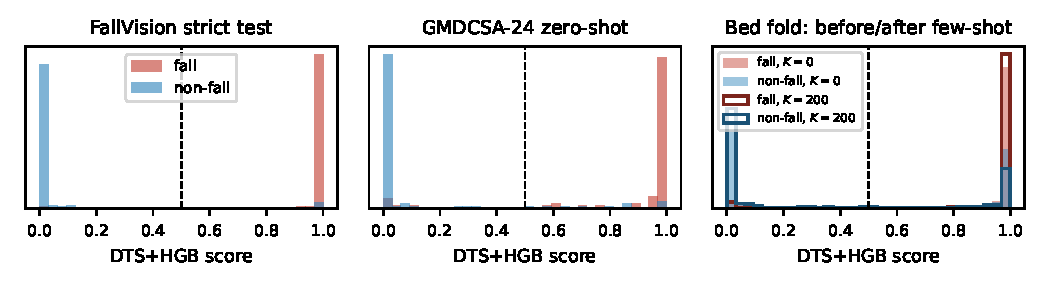
\includegraphics[width=0.95\textwidth]{fig_score_dists.pdf}
\caption{Class-conditional DTS+HGB score distributions from the saved score vectors (dashed line: fixed threshold 0.5). Left: FallVision strict test (well calibrated). Centre: GMDCSA-24 zero-shot (default threshold usable; 12.3\% non-fall mass above 0.5). Right: the hard Bed fold before ($K{=}0$, filled) and after ($K{=}200$, outlined) few-shot adaptation, which thins the high-score non-fall mass and widens the fall/non-fall separation from 0.44 to 0.59.}
\label{fig:scoredists}
\end{figure}

\begin{table}[h]
\centering
\small
\setlength{\tabcolsep}{3.4pt}
\begin{tabular}{lccc}
\toprule
Metric & FallVision (test) & URFD & GMDCSA-24 \\
\midrule
AUROC & 0.9895 [0.985, 0.994] & 0.9200 [0.848, 0.992] & 0.9633 [0.936, 0.985] \\
Recall & 0.969 [0.953, 0.983] & 1.000 [0.886, 1.000] & 0.924 [0.844, 0.965] \\
Precision & 0.934 [0.913, 0.954] & 0.508 [0.384, 0.632] & 0.880 [0.792, 0.933] \\
F1 & 0.951 [0.938, 0.963] & 0.674 [0.550, 0.779] & 0.901 [0.848, 0.947] \\
FN & 18 & 0 & 6 \\
FP & 39 & 29 & 10 \\
\bottomrule
\end{tabular}
\caption{Zero-shot cross-dataset transfer for DTS+HGB (FallVision-trained, fixed threshold 0.5): URFD (70 clips) and the uncontrolled-home GMDCSA-24 (160 clips). AUROC/F1 use bootstrap intervals (URFD AUROC: Hanley--McNeil, as no score vector was retained from the archived run); recall and precision use Wilson count intervals; FP and FN are deterministic counts.}
\label{tab:transfer}
\end{table}

\begin{figure}[h]
\centering
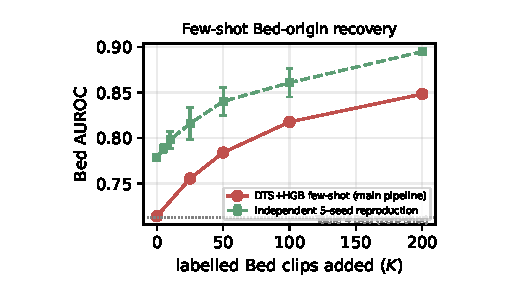
\includegraphics[width=0.6\columnwidth]{fig2_bed_recovery.pdf}
\caption{Original few-shot Bed-origin recovery: main-pipeline curve and an independent five-seed re-implementation (95\% intervals); both recover the fold monotonically. The matched-protocol baseline comparison is in main-text Figure~\ref{fig:bed}.}
\label{fig:bedorig}
\end{figure}

\begin{table}[h]
\centering
\small
\begin{tabular}{lccccc}
\toprule
Model & S1 & S2 & S3 & S4 & Mean \\
\midrule
DTS+HGB & 0.953 & 0.969 & 0.970 & 0.871 & \textbf{0.941} \\
MultiROCKET & 0.988 & 0.882 & 0.948 & 0.918 & 0.934 \\
MiniROCKET & 0.988 & 0.816 & 0.942 & 0.926 & 0.918 \\
$\alpha$-only+LR & 0.977 & 0.944 & 0.965 & 0.782 & 0.917 \\
\bottomrule
\end{tabular}
\caption{True leave-one-subject-out AUROC on GMDCSA-24 (4 subjects). DTS+HGB matches the strong modern convolutional time-series baseline MultiROCKET under person-level shift, with a small, non-significant mean-AUROC advantage.}
\label{tab:loso}
\end{table}

\begin{table}[h]
\centering
\small
\begin{tabular}{lllcc}
\toprule
Analysis & Test subset & Seeds & DTS $K{=}0$ & DTS $K{=}200$ \\
\midrule
Leave-fall-origin (zero-shot) & full Bed fold (1,747) & 1 & 0.7123 & -- \\
Original adaptation & reserved Bed test & main run & 0.714 & 0.848 \\
Independent reproduction & reserved Bed test & 5 & 0.778 & 0.895 \\
Matched 3-way (Figure~\ref{fig:bed}) & fixed 1,547 clips & 5 & 0.715 & 0.858 \\
\bottomrule
\end{tabular}
\caption{Mapping of every Bed-recovery number to its protocol; values differ because the analyses use different Bed test subsets and seed counts. In the matched 3-way comparison (Figure~\ref{fig:bed}), at $K{=}0\rightarrow200$ DTS+HGB goes 0.715$\rightarrow$0.858, MiniROCKET 0.714$\rightarrow$0.825, and MultiROCKET 0.758$\rightarrow$0.864: DTS+HGB leads MiniROCKET throughout and is marginally trailed by MultiROCKET.}
\label{tab:bedmap}
\end{table}

\subsection{Paired Learning-Curve Comparison}
Table~\ref{tab:lcpaired} reports the paired bootstrap of the DTS+HGB$-$MultiROCKET AUROC difference at each training size (identical stratified subsamples and test resamples; 1,000 resamples, fixed seed; both models retrained per size in the same harness). No difference is significant at any size.

\begin{table}[h]
\centering
\small
\begin{tabular}{lcccc}
\toprule
$n$ & DTS+HGB & MultiROCKET & paired $\Delta$ & 95\% CI \\
\midrule
250 & 0.9477 & 0.9501 & $-0.0024$ & [$-0.0163$, $+0.0101$] \\
500 & 0.9618 & 0.9578 & $+0.0039$ & [$-0.0058$, $+0.0149$] \\
1{,}000 & 0.9732 & 0.9737 & $-0.0005$ & [$-0.0085$, $+0.0080$] \\
2{,}000 & 0.9828 & 0.9788 & $+0.0040$ & [$-0.0022$, $+0.0117$] \\
3{,}565 & 0.9895 & 0.9868 & $+0.0027$ & [$-0.0027$, $+0.0090$] \\
\bottomrule
\end{tabular}
\caption{Paired learning-curve comparison on the strict twin-free split. All five intervals contain zero: the two methods are not significantly different at any training size, while both dominate the learned sequence models (Figure~\ref{fig:sampleeff}).}
\label{tab:lcpaired}
\end{table}

\subsection{Leave-Session-Out (Subject Proxy)}
With no published FallVision subject IDs, the four archive-derived sessions serve as a coarse subject proxy. DTS+HGB attains mean AUROC 0.9649 (range 0.9382--0.9926) over the four folds, consistent with the true subject-held-out result on GMDCSA-24.

\begin{table}[h]
\centering
\small
\begin{tabular}{lccccc}
\toprule
Session & $n$ & Falls & F1 & AUROC & Recall \\
\midrule
1 & 1,513 & 679 & 0.866 [0.847, 0.884] & 0.9382 [0.9259, 0.9492] & 0.944 \\
2 & 1,593 & 1,072 & 0.966 [0.958, 0.973] & 0.9926 [0.9898, 0.9951] & 0.954 \\
3 & 2,064 & 903 & 0.925 [0.912, 0.937] & 0.9840 [0.9797, 0.9879] & 0.925 \\
4 & 402 & 213 & 0.868 [0.836, 0.900] & 0.9448 [0.9227, 0.9645] & 0.953 \\
\midrule
Mean & -- & -- & 0.906 & 0.9649 & -- \\
\bottomrule
\end{tabular}
\caption{Leave-session-out evaluation for DTS+HGB (subject proxy; fixed threshold 0.5). Brackets are 95\% bootstrap confidence intervals.}
\label{tab:lso}
\end{table}

\subsection{Leave-Fall-Origin Detail and Capacity Reference Scale}
Table~\ref{tab:lfo} gives the per-origin folds behind the leave-fall-origin analysis; Figure~\ref{fig:capacity} plots the heuristic capacity comparison of Proposition~\ref{prop:capacity}.
\begin{table}[h]
\centering
\small
\begin{tabular}{lcccc}
\toprule
Held-out & $n$ & Falls & F1 & AUROC \\
\midrule
Bed & 1,747 & 922 & 0.768 [0.749, 0.788] & 0.7123 [0.6868, 0.7357] \\
Chair & 1,878 & 961 & 0.934 [0.923, 0.944] & 0.9844 [0.9799, 0.9883] \\
Stand & 1,947 & 984 & 0.937 [0.926, 0.949] & 0.9916 [0.9886, 0.9945] \\
\midrule
Mean & -- & -- & 0.880 & 0.8961 \\
\bottomrule
\end{tabular}
\caption{Leave-fall-origin robustness for DTS+HGB (fixed threshold 0.5). Brackets are 95\% bootstrap confidence intervals.}
\label{tab:lfo}
\end{table}

\begin{figure}[h]
\centering
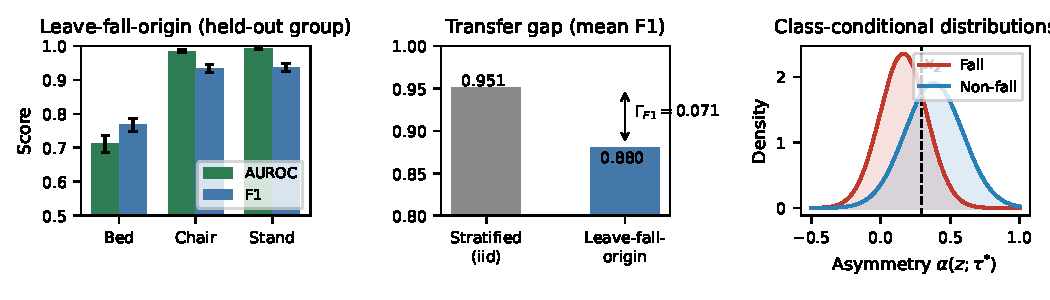
\includegraphics[width=0.98\textwidth]{fig4_lfo_panels.pdf}
\caption{Left: leave-fall-origin AUROC and F1 by held-out acquisition group with 95\% confidence intervals. Centre: transfer gap between the stratified iid reference and the leave-fall-origin mean under the same protocol ($\Gamma_{F1}=0.951-0.880=0.071$). Right: class-conditional distributions of hip-speed asymmetry (training-only estimates on the corrected data) with the active QDA boundary $x_2\approx0.293$; the lower crossover lies outside the support of $\alpha$.}
\label{fig:lfopanels}
\end{figure}

\begin{figure}[h]
\centering
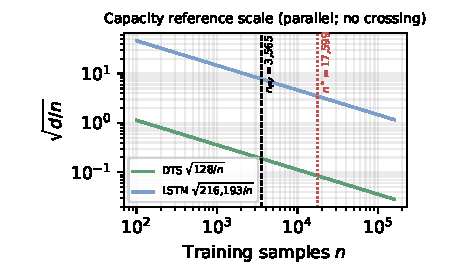
\includegraphics[width=0.55\textwidth]{fig5_capacity.pdf}
\caption{Heuristic capacity comparison (Proposition~\ref{prop:capacity}): the $\sqrt{d/n}$ curves for DTS and the LSTM are parallel and do not cross; $n^{*}\approx17{,}599$ (dotted) is a derived reference scale and $n_{\mathrm{train}}=3{,}565$ (dashed) lies well below it.}
\label{fig:capacity}
\end{figure}

\subsection{Hyperparameter Grids and Feature Ablations}
Table~\ref{tab:grids} lists the validation-only search grids and selected configurations for the DTS classifiers and MiniROCKET; neural baseline architectures are fixed a priori (main text).

\begin{table}[h]
\centering
\small
\begin{tabular}{lll}
\toprule
Model & Search space & Selected \\
\midrule
DTS+LR & $C\in\{0.05,0.1,0.5,1,2,10\}$ & $C{=}0.05$ \\
DTS+ET & trees $\{100,300,600\}\times$ feat.\ $\{\sqrt{d},0.25\}$ & 100 trees, max\_features${=}0.25$ \\
DTS+RF & trees $\{100,300,600\}\times$ feat.\ $\{\sqrt{d},0.25\}$ & 600 trees, max\_features${=}0.25$ \\
DTS+HGB & iter.\ $\{100,300,600\}\times$ lr $\{0.05,0.1,0.2\}\times\lambda_2\{0,0.1\}$ & 600 iterations, lr${=}0.1$, $\lambda_2{=}0.1$ \\
MiniROCKET & kernels $\{1000,5000,10000\}$ & 10,000 \\
\bottomrule
\end{tabular}
\caption{Hyperparameter grids and validation-selected configurations for the DTS classifiers and MiniROCKET. Neural baseline architectures are fixed a priori (see text); their decision thresholds are tuned on validation F1 like all other models.}
\label{tab:grids}
\end{table}

Table~\ref{tab:ablation} gives the per-family single-removal and asymmetry-zeroed ablation discussed in the main text.
\begin{table}[h]
\centering
\small
\begin{tabular}{lcccc}
\toprule
Configuration & F1 & AUROC & $\Delta$F1 & $\Delta$AUC \\
\midrule
Full model & 0.951 & 0.9895 & -- & -- \\
$-$BBox-W & 0.942 & 0.9882 & $-0.009$ & $-0.0013$ \\
$-$Hip-Y & 0.939 & 0.9855 & $-0.012$ & $-0.0039$ \\
$-$Torso-Ang & 0.945 & 0.9892 & $-0.006$ & $-0.0003$ \\
$-$Hip-Spd & 0.949 & 0.9897 & $-0.002$ & $+0.0002$ \\
$-$Ctr-Spd & 0.949 & 0.9904 & $-0.002$ & $+0.0009$ \\
$-$Hip-Acc & 0.947 & 0.9894 & $-0.004$ & $-0.0001$ \\
$-$Shldr-Y & 0.943 & 0.9882 & $-0.008$ & $-0.0012$ \\
$-$Head-Y & 0.951 & 0.9903 & $-0.001$ & $+0.0008$ \\
Asymmetry zeroed ($\alpha{=}0$) & 0.939 & 0.9872 & $-0.012$ & $-0.0023$ \\
\bottomrule
\end{tabular}
\caption{DTS+HGB feature ablation on the main held-out protocol (each row retrained; threshold re-tuned on validation). Values to three decimals (F1) and four decimals (AUROC).}
\label{tab:ablation}
\end{table}

\subsection{Expanded Controlled-Benchmark Sweeps}
\begin{table}[t]
\centering
\small
\setlength{\tabcolsep}{4pt}
\begin{tabular}{lccc}
\toprule
Model & Fall & Sit-to-stand & Reversal \\
\midrule
DTS+HGB (128-d) & 1.000 & 1.000 & 1.000 \\
$\alpha$-only+LR (8-d) & 1.000 & 1.000 & 1.000 \\
MiniROCKET+Ridge & 1.000 & 1.000 & 1.000 \\
Raw-seq MLP & 1.000 & 1.000 & 1.000 \\
Bag-of-frames+HGB & 0.500 & 0.500 & 0.500 \\
\bottomrule
\end{tabular}
\caption{Expanded controlled temporal-order benchmark: held-out AUROC (mean$\pm$sd over five seeds, $n{=}250$ training pairs, 500 test pairs) on three constructions whose negatives are frame permutations (Fall, Sit-to-stand) or exact time reversals (Reversal) of positives, so class-conditional frame multisets are identical and Theorem~\ref{thm:impossibility} applies. Order-invariant bag-of-frames is exactly at chance everywhere; the structured signature and order-sensitive baselines solve all three constructions. Full $n$-sweeps in the appendix artefacts.}
\label{tab:bench}
\end{table}

\begin{figure}[t]
\centering
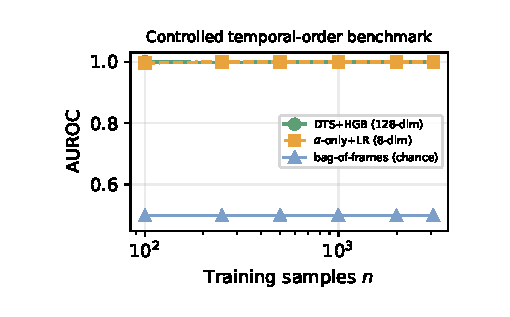
\includegraphics[width=0.5\textwidth]{fig3_controlled_benchmark.pdf}
\caption{Original controlled temporal-order benchmark: DTS+HGB and asymmetry-only saturate, while the order-invariant bag-of-frames classifier sits exactly at chance for every $n$ (Theorem~\ref{thm:impossibility}), the two classes having identical marginals by construction.}
\label{fig:benchmark}
\end{figure}

\begin{table}[h]
\centering
\small
\begin{tabular}{lcccc}
\toprule
Setting & DTS+HGB & $\alpha$-only+LR & Bag-of-frames & MiniROCKET \\
\midrule
\multicolumn{5}{l}{\emph{Drop SNR $\mu_d/\sigma_s$ (fall, $n{=}250$)}} \\
SNR 1 & 1.000 & 0.879{\scriptsize$\pm$0.004} & 0.500 & 1.000 \\
SNR 2 & 1.000 & 0.993{\scriptsize$\pm$0.001} & 0.500 & 1.000 \\
SNR 4 & 1.000 & 1.000 & 0.500 & 1.000 \\
SNR 8 & 1.000 & 1.000 & 0.500 & 1.000 \\
SNR 16 & 1.000 & 1.000 & 0.500 & 1.000 \\
\midrule
\multicolumn{5}{l}{\emph{Event onset $p_1$ (fall, $n{=}250$)}} \\
$p_1{=}0.15$ & 1.000 & 1.000 & 0.500 & -- \\
$p_1{=}0.3$ & 1.000 & 1.000 & 0.500 & -- \\
$p_1{=}0.5$ & 1.000 & 1.000 & 0.500 & -- \\
$p_1{=}0.7$ & 1.000 & 1.000 & 0.500 & -- \\
\midrule
\multicolumn{5}{l}{\emph{$\alpha$-only with misspecified fixed $\tau{=}0.30$ vs train-selected $\tau$}} \\
$p_1{=}0.15$ & \multicolumn{2}{c}{selected: 1.000} & \multicolumn{2}{c}{fixed 0.30: 1.000} \\
$p_1{=}0.3$ & \multicolumn{2}{c}{selected: 1.000} & \multicolumn{2}{c}{fixed 0.30: 0.993{\scriptsize$\pm$0.001}} \\
$p_1{=}0.5$ & \multicolumn{2}{c}{selected: 1.000} & \multicolumn{2}{c}{fixed 0.30: 1.000} \\
$p_1{=}0.7$ & \multicolumn{2}{c}{selected: 1.000} & \multicolumn{2}{c}{fixed 0.30: 0.999} \\
\midrule
\multicolumn{5}{l}{\emph{Distractor channels added (fall, $n{=}250$)}} \\
+0 noise ch. & 1.000 & 1.000 & 0.500 & 1.000 \\
+8 noise ch. & 1.000 & 1.000 & 0.500 & 1.000 \\
+32 noise ch. & 1.000 & 1.000 & 0.500 & 1.000 \\
+120 noise ch. & 1.000 & 1.000 & 0.500 & 1.000 \\
\midrule
\multicolumn{4}{l}{\emph{Event duration $p_2{-}p_1$ (fall, $n{=}250$)}} \\
dur 0.05 & 1.000 & 0.992{\scriptsize$\pm$0.001} & 0.500 \\
dur 0.1 & 1.000 & 0.999 & 0.500 \\
dur 0.2 & 1.000 & 1.000 & 0.500 \\
dur 0.4 & 1.000 & 1.000 & 0.500 \\
\midrule
\multicolumn{4}{l}{\emph{Sequence length $T$ (fall, $n{=}250$)}} \\
$T{=}30$ & 1.000 & 0.999 & 0.500 \\
$T{=}60$ & 1.000 & 1.000 & 0.500 \\
$T{=}150$ & 1.000 & 1.000 & 0.500 \\
$T{=}300$ & 1.000 & 1.000 & 0.500 \\
\midrule
\multicolumn{5}{l}{\emph{Operator-bank ablation, DTS+HGB (fall, $n{=}250$)}} \\
full 16-operator bank & \multicolumn{4}{c}{1.000} \\
$-$ all $\alpha$ & \multicolumn{4}{c}{1.000} \\
$\alpha$ only & \multicolumn{4}{c}{1.000} \\
order-sensitive ops only & \multicolumn{4}{c}{1.000} \\
order-invariant ops only & \multicolumn{4}{c}{0.500} \\
quantiles/min/max only & \multicolumn{4}{c}{0.500} \\
slopes only & \multicolumn{4}{c}{1.000} \\
endpoints only & \multicolumn{4}{c}{0.997{\scriptsize$\pm$0.002}} \\
\bottomrule
\end{tabular}
\caption{Controlled-benchmark sweeps (held-out AUROC, mean$\pm$sd over three seeds, 500 test pairs). Bag-of-frames remains at exactly 0.500 in every setting, as Theorem~\ref{thm:impossibility} requires, and order-invariant operator subsets of the signature itself (quantiles, min/max) also sit exactly at chance, confirming that the order-sensitive operators carry all discriminative signal. $\alpha$-only degrades as drop SNR approaches 1 and dips mildly under a misspecified fixed $\tau$ or very short events, while the full operator bank and train-selected $\tau$ remain at ceiling. At these settings every order-sensitive method solves the constructions, including with 120 distractor channels: the family measures the necessity of order sensitivity, not separation among order-sensitive methods.}
\label{tab:benchsweeps}
\end{table}


All sweep configurations, seeds, per-run results, and the exact generator code are released (\texttt{synth\string_bench.py}, \texttt{results\_all.jsonl}). Construction defaults: $T{=}150$, eight informative channels, drop SNR 8, event onset $p_1{=}0.5$ (fall) / $0.4$ (sit-to-stand), duration $0.2$ (fall) / $0.3$ (sit-to-stand), 500 held-out test pairs per run; $\tau$ selected on training data only by the summed-Welch rule. The bag-of-frames feature map is per-channel value quantiles, order-invariant by construction.

\end{document}
